\documentclass{article}
\usepackage{amsmath}
\usepackage{tikz}

\begin{document}

The computational model consists of a computing machine (any physical object) \( M \) described by a set of complex differential operators \( \mathbf{L} \). \( | \mathbf{f} \rangle \) and \( \mathbf{L} | \mathbf{f} \rangle = | \mathbf{f}' \rangle \) are the inputs and outputs analytic complex functions.

\begin{center}
    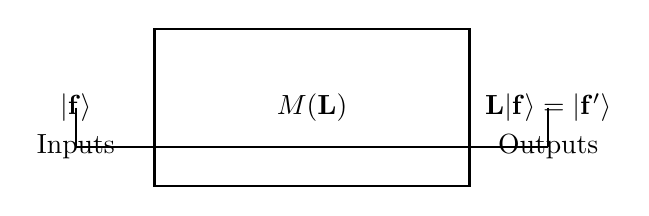
\begin{tikzpicture}[scale=1]
        % Draw the box for the computing machine
        \draw[thick] (0,0) rectangle (4,2);
        
        % Label the inputs
        \node at (-1, 1) {$| \mathbf{f} \rangle$};
        \node at (-1, 0.5) {Inputs};
        
        % Label the outputs
        \node at (5, 1) {$\mathbf{L} | \mathbf{f} \rangle = | \mathbf{f}' \rangle$};
        \node at (5, 0.5) {Outputs};
        
        % Draw the lines connecting the inputs and outputs
        \draw[thick] (-1, 1) -- (-1, 0.5);
        \draw[thick] (5, 1) -- (5, 0.5);
        \draw[thick] (-1, 0.5) -- (5, 0.5);
        
        % Label the machine
        \node at (2, 1) {$M(\mathbf{L})$};
    \end{tikzpicture}
\end{center}

\end{document}